
\section{LBNF Experimental Setup}
% Need to be approximately 7 pages:
% 1 page for general words
% 2 pages for neutrino beam, near detector and far detector

The Long Beamline Neutrino Facility (LBNF) is the facility being internationally designed for the future Deep Underground Neutrino Experiment (DUNE) for the precision measurements of neutrino oscillations parameters and related searches beyond the Standard Model. The general scheme of the facility is shown on figure \ref{fig:LBNF_overallScheme}. The first collaboration meeting took place on April 16th-18th of 2015 in Fermilab \cite{ref_LBNF_collaborationMeeting}. There were about 200 participants out of total of 750 members. The statuses and prospectives of the Near Detector, Far Detector, Neutrino beam, software infrastructure and other related technical topics were discussed. Most information written in this section is taken from the presentations of this collaboration meeting, the Concettual Design Report (CDR) drafts \cite{ref_LBNFdoc_volume-detectors}, \cite{ref_LBNFdoc_volume-physics} and the main pages of the LFNF website \cite{ref_LBNFweb}.

\begin{figure}
\caption{The Fermilab Accelerator Complex as it is described in the presentation "The LBNF Beamline and PIP-II" by Vaia Papadimitriou at the fisrt LBNF Collaboration meeting \cite{ref_LBNF_collaborationMeeting}}
\label{fig:LBNF_FermilabAccComplex}
\centering
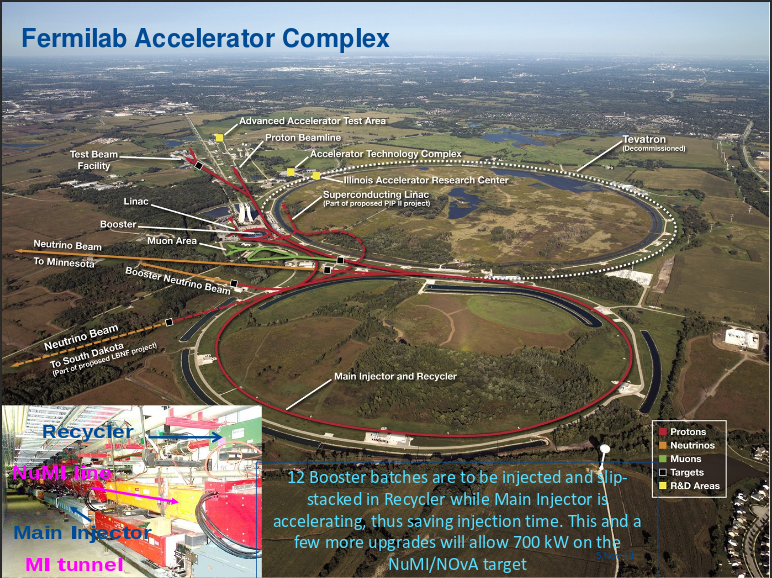
\includegraphics[width=0.95\textwidth, keepaspectratio=true]{figs/FermilabAccelerator.png}

\end{figure}

\begin{figure}
\caption{Long Baseline Neutrino Facility (LBNF). The neutrino flux will be produced using existing proton accelerator in Fermilab. Then neutrinos will be registered by near detector, travel 1300 km through the Earth mantle to the Sanford Underground Research Facility in South Dakota and be registed by far detector. Source of figure: \cite{ref_LBNFweb} }
\label{fig:LBNF_overallScheme}
\centering
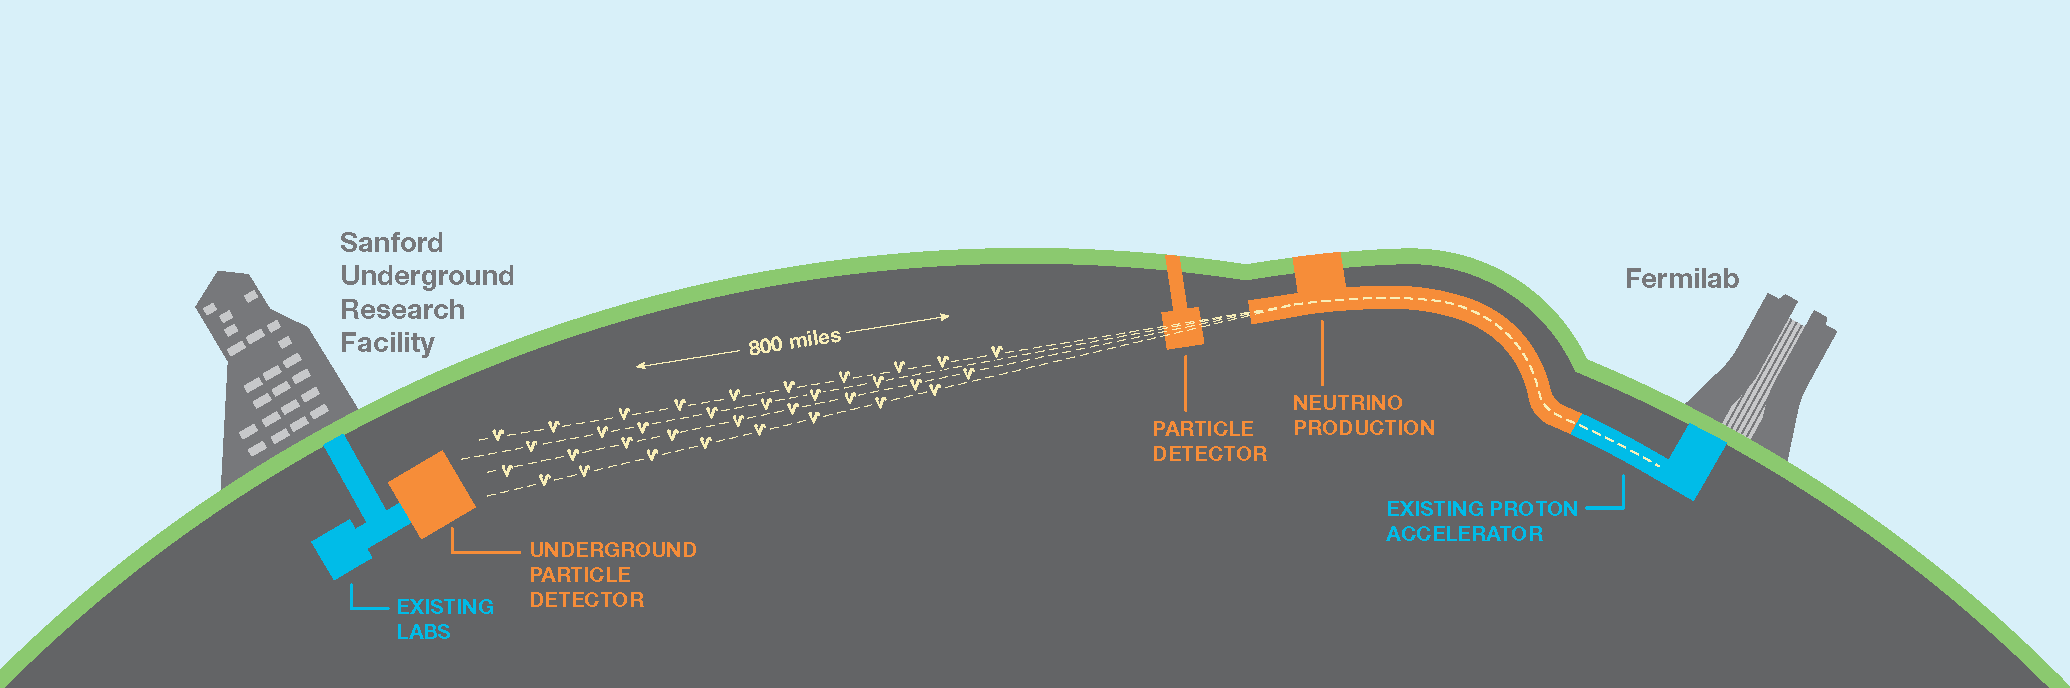
\includegraphics[width=0.95\textwidth, keepaspectratio=true]{figs/LBNF_overallScheme.png} 
\end{figure}

Scheme of the Fermilab accelerator complex is shown at the (fig. \ref{fig:LBNF_FermilabAccComplex} ) and the overall scheme of the 
Long Baseline Neutrino Facility (LBNF) is shown at the (fig. \ref{fig:LBNF_overallScheme} ). The protons from the accelerator  will induce the neutrino beam which will be travel trough the Earth in direction of the Deep Underground Neutrino Experiment (DUNE) detector in South Dakota. It is common for the long baseline neutrino oscillations experiments to have a near detector (several hundred meters from the neutrino production) and far detector (hundreds of kilometers away). Comparing measurements of neutrino flux characteristics at two points allows to extract parameters of neutrino oscillations physics.

General requirements for the experiment are listed in \cite{ref_LBNFdoc_volume-detectors}.
\begin{itemize}
  \item neutrino beam of high intensity which would be able to produce large amount of neutrinos to be registered at the far site
  \item the detector to register neutrinos and measure the beamline characteristics at the near site
  \item the liquid argon time-projection chamber for the far site detector (LArTPC)
\end{itemize}

\subsection{Neutrino Beam}

\begin{figure}
\caption{The neutrino beam production at the LBNF. Source of figure: \cite{ref_LBNFweb}}
\label{fig:LBNF_nuBeam}
\centering
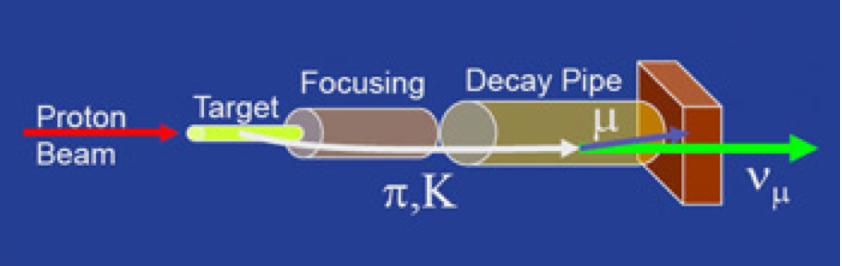
\includegraphics[width=0.45\textwidth, keepaspectratio=true]{figs/LBNF_nuBeam.png}  
\end{figure}


\begin{figure}
\caption{Examples of the Feynmann diagrams of charged pion and kaon productions in proton-proton scattering.}
\label{fig:pionAndKaonProductions}
\centering
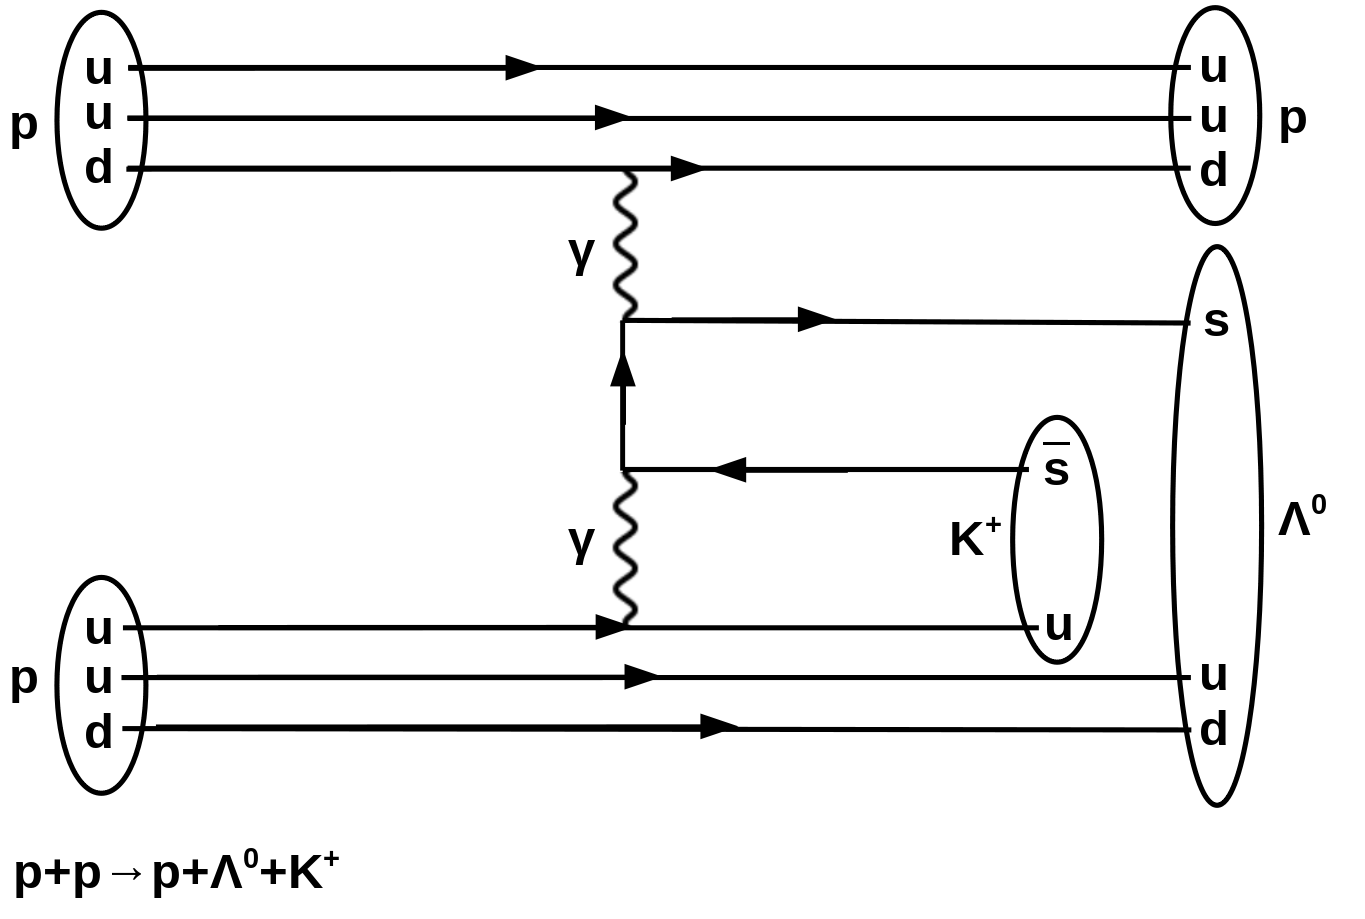
\includegraphics[width=0.48\textwidth, keepaspectratio=true]{figs/ppKaonProduction.png}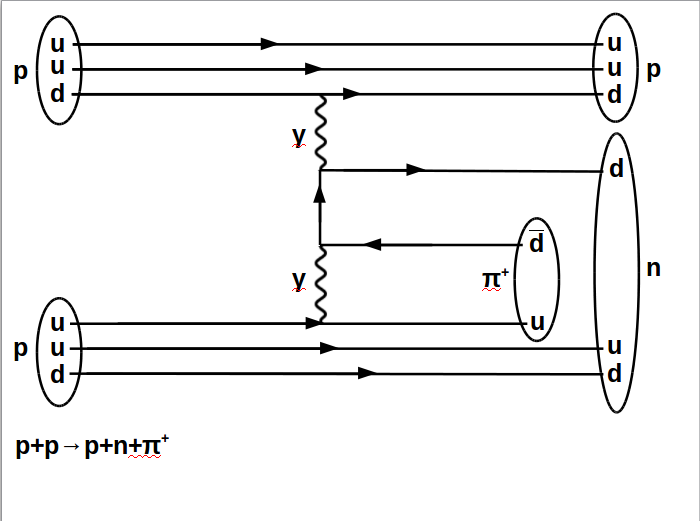
\includegraphics[width=0.48\textwidth, keepaspectratio=true]{figs/ppPionProduction.png}  
\end{figure}


The LBNF neutrino beam will be the highest intensity neutrino beam ever created. The proton accelerator in Fermilab which was already used in other experiments in Fermilab before will produce the beam of protons. Then protons will hit a target and create kaons and pions through the same reactions as take place in atmosphere when the cosmic protons hit molecules of air.  Pions can be created in the reactions $p+p \rightarrow p+n+\pi^+$, $p+p \rightarrow p+\Delta^{++}+\pi^-$, $p+n \rightarrow p+p+\pi^-$, $p+n \rightarrow n+n+\pi^+$, $p+n \rightarrow p+\Delta^{-}+\pi^+$ etc which go electromagnetically though photon. In more general words, one quark from the accelerator beam proton scatters on the other quark from the proton or neutron of the target substance as shown at fig. \ref{fig:pionAndKaonProductions}. They exchange photon which produces quark-antiquark pair. At this moment, the system has seven quarks and one antiquark. The antiquark pairs up with one of the quarks participating in the reaction and the remaining six quarks make two baryons.  The charged pions have formulas $\pi^+ = u\bar{d}$ and $\pi^- = \bar{u}d$ and can be produced with the reactions which only include first generation quarks. The formulas of charged kaons are $K^+ = u\bar{s}$, $K^- = \bar{u}s$. Thus, to produce kaons, the photon has to produce $s\bar{s}$ pair. 

\begin{figure}
\caption{Feynmann diagrams of charged pion and kaon decays to muon and muon antineutrino weakly through W-boson. Figures taken from \cite{ref_fig_pionandKaonDecays}.}
\label{fig:pionAndKaonDecays}
\centering
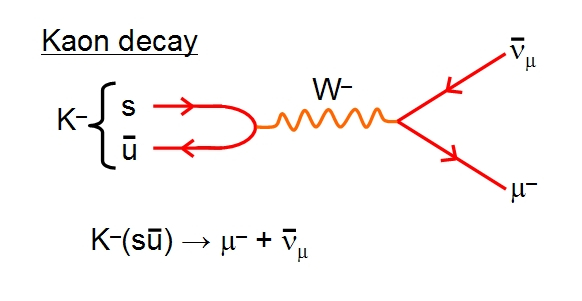
\includegraphics[width=0.45\textwidth, keepaspectratio=true]{figs/kaonDecay.jpg}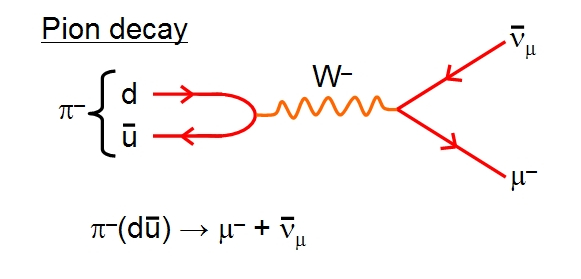
\includegraphics[width=0.45\textwidth, keepaspectratio=true]{figs/pionDecay.jpg} 
\end{figure}

After the mesons are created, they go through the focusing camera and decay into the decay pipe (the length of the decay pipe is about 200 meters) as $\pi^+ \rightarrow \mu^+\nu_\mu$, $\pi^- \rightarrow \mu^-\bar{\nu_\mu}$, $K^+ \rightarrow \mu^+\nu_\mu$, $K^- \rightarrow \mu^-\bar{\nu_\mu}$ (fig. \ref{fig:pionAndKaonDecays}). The branching ratios of charged pions and kaons to decay into $\mu^+\nu_\mu$($\mu^-\bar{\nu_\mu}$) are $(>99.9)\%$ and $(63.55\pm0.011)\%$ respectively therefore most neutrinos produced into the decay pipe will be muon neutrinos. (While the neutral kaons can also be produced in the target and later decay in pions which could further decay and produce muon neutrinos, the focusing is being done with the certain configuration of the magnetic field and only can affect charged particles. Neutral pions, $\pi^0$s, are very likely to be produced as well but they decay as $\pi^0 \rightarrow \gamma\gamma$ and, therefore. can't contribute to the neutrino production.)

After being produced in the reactions described above, the neutrinos will be detected in the near detector in the Fermilab. Then the neutrinos will travel 1300 km through the Earth crust and will be detected by Sanford Underground Research Facility in South Dakota.\\*  

Beam requirements listed in the "Beam Requirements and Beam Optimization talk" during the first LBNF collaboaration meeting include:
\begin{itemize}
  \item the beam must have high intensity, be wide-band
  \item must be able to produce muon neutrinos or antineutrinos by experimenter's choice
  \item fraction of the opposite sign neutrinos must be small
  \item the energy range of the first oscillation node (1-5 GeV) must be fully covered
  \item the second oscillation node, $\sim{0.8}$ GeV must be achievable too
  \item must work at $>\sim{2} $ MW at 60-120 GeV/c
  \item the option to tune the lower primary proton momenta down to 60 GeV/c must present
  \item the parameters of the neutrino flux must be stable
\end{itemize}

\subsection{Near Detector}


A near detector is an important part of any long baseline neutrino oscillation experiment. It measures the primary neutrino beam flux as it is produced by the beam production system. Chapter 6 of the draft LBNF CDR \cite{ref_LBNFdoc_volume-detectors} lists the following precision measurements to be performed by the Near Detector: 
\begin{itemize}
  \item absolute flux measurement
  \item relative neutrino and antineutrino flux measurements
  \item flavor content of the neutrino source
  \item determination of the $E_\nu$-scale of neutrinos versus antineutrinos
  \item event-by-event measurements of NC interactions
  \item measurement of $\pi^0$, $\pi^\pm$, $K^\pm$, p, $K^0_S$ and $\Lambda$ in the NC and CC
%  \item "quasi-elastic and resonance measurements"
  \item nucleon structure, parton distribution functions and QCD studies
%  \item neutrino-argon interactions and nuclear effects
  \item precision measurements of electroweak physics
%  \item isospin physics and the Adler sum rule
%  \item measurement of the nuclean strangeness content
\end{itemize}

More specifically, the list of the physics measurements related to the neutrino oscillations to be performed by the Near Detector includes:
\begin{itemize}
  \item fluxes of $\nu_\mu$, $\bar{\nu_\mu}$, $\nu_e$ and $\bar{\nu_e}$. To distinguish between flavors, the measurement should rely on charged current interaction (fig. \ref{fig:MuonAndNeutronDecays}, middle and right) and measure the products of these interactions $\mu^-$, $\mu^+$, $e^-$, and $e^+$. (While the beam production system has the highest probability to produce muon neutrinos, the production of certain number electron neutrinos is also possible, for example, from charged kaon decays)
  \item $\nu_e$-$\bar{\nu_e}$ assymetries. For that, it's important not only distinguish between $\mu^\pm$ and $e^\pm$ but also between $e^-$ and $e^+$.
  \item the absolute $\nu_\mu$ and $\bar{\nu_\mu}$ fluxes need to be measured with $\simeq{3\%}$ precision in the neutrino energy range 0.5-8 GeV
  \item cross section of NC versus CC processes as a function of hadronic energy. NC is one of major backrounds which contribute to neutrino oscillation measurement
  \item yields of $\pi_0$ and photons. These particles are the most significant background to $\nu_e$ and $\bar{\nu_e}$ contamination
  \item fractions of the $\pi^\pm$ into the CC and the NC hadronic jets.    
\end{itemize} 

%\begin{SCfigure}
%side caption
%\caption{Scheme of the Near Detector. The detector will consist of central Straw-Tube Tracker (STT) modules, electromagnetic calorimeter (ECAL), magnet coils of 0.4T and muon identification system consisting of Resistive Plate Chamber (RPC) modules. The neutrinos would come from the bottom left corner of the picture, to the End RPCs. Source of figure: [REFERENCE]}
%\label{fig:nearDetector}
%\centering
%\includegraphics[width=0.50\textwidth, keepaspectratio=true]{figs/%nearDetector.png}
%\end{SCfigure}

\begin{figure}
\caption{Scheme of the DUNE Near Detector (left) and related complex (right).}
\label{fig:nearDetector}
\centering
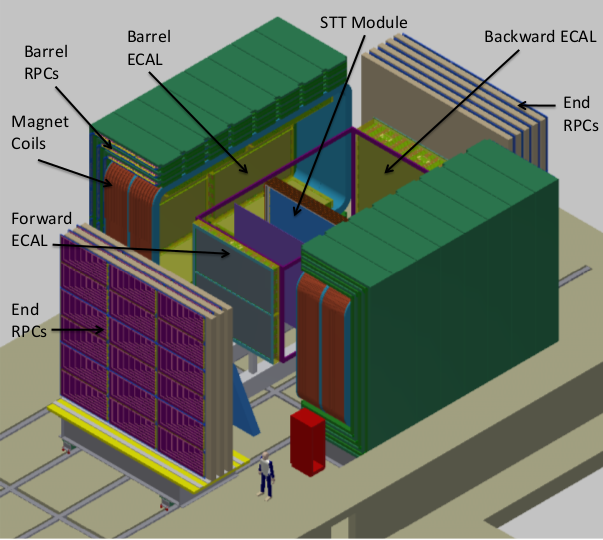
\includegraphics[width=0.63\textwidth, keepaspectratio=true]{figs/nearDetector.png}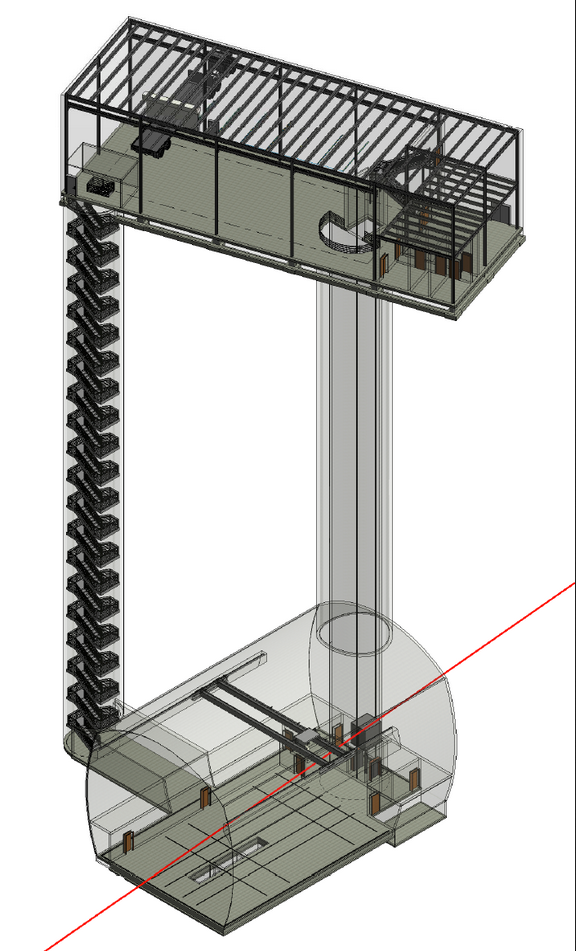
\includegraphics[width=0.35\textwidth, keepaspectratio=true]{figs/nearDetector_project.png}
\end{figure}

The scheme of the near detector is shown at the fig. \ref{fig:nearDetector}. The detector will consist of central Straw-Tube Tracker (STT) modules, electromagnetic calorimeter (ECAL), magnet coils of 0.4T and muon identification system consisting of Resistive Plate Chamber (RPC) modules. The neutrinos would come from the bottom left corner of the picture, to the End RPCs.

Quoting the LBNF website \cite{ref_LBNFweb}, "The DUNE near detector will require LBNF to excavate and provision a cavern 200 ft (60 m) below grade on the Fermilab site and to construct a surface building directly above it. An elevator will provide the primary access between the two spaces; the stairway shown is planned for emergency egress. This complex will be constructed a minimum of 690 feet (210 m) downstream of the beamline target."

\subsection{Far Detector}

The LBNF website \cite{ref_LBNFweb} provides general description of the DUNE far detector which to be located at Sanford Undergroud Research Facility (SURF) in South Dakota. General view pictures of the facility are shown at fig. \ref{fig:farDetector_SURF1} and fig. \ref{fig:farDetector_SURF2}. There will be four modules, 10,000 tonnes of liquid argon each placed into four caverns 1500 m underground. Each module will be 15 m wide, 12 m high and 58 m long, along the beam direction. The caverns will be placed as pairs and there will be the fifth cavern between two pairs - the one with the cryogenic equipment, to provide cooling for 89K liquid argon and to keep agron pure and circulating smoothly during operations. 
That's how Tia Miceli, postdoctoral reaseacher at New Mexico State University, in her article for the "Fermilab today" \cite{ref_aboutLAr} explains why liquid argon is excellent working substance for neutrino detectors:
"For particle physics, perhaps liquid argon's most important feature is that it acts as both a target and detector for neutrinos $<...>$ With 40 protons and neutrons, liquid argon is denser than water or oil, so liquid-argon detectors see more neutrino collisions per unit volume than their oil- or water-based predecessors. That means faster measurements and consequently faster discoveries. Another advantage of liquid argon is that, when a neutrino interacts with it and subsequently generates charged particles, it produces two separate kinds of signals; oil- or water-based detectors produce only one. One type of signal, unique to liquid argon, results from its ability to record the charged particles' trajectories. Charged particles are created in the liquid argon after a neutrino flies in and collides with an argon nucleus. The charged debris travels through the argon and easily knocks off electrons from the neighboring atoms along its path. The electronic traces in the liquid argon are pushed by an applied electric field toward an array of wires (similar to a guitar's) on the side of the detector. The wires collect data on the particle trajectories, producing a signal. The second signal type is one shared with oil- and water-based detection: a flash of light. When a charged particle bumps into an argon atom's electron, the electron transitions to a higher energy. As the electron transitions back to its original state, the excess energy is emitted as light. 
It turns out that argon is also relatively cheap. Companies liquefy air and heat it slowly. Since each of air's components has a unique boiling temperature, they can be separated. The boiled-off argon is moved to a separate chamber where it is again condensed. The commercially available liquid argon that we buy is still not pure enough for our experiments, so once the liquid argon arrives at the lab, we filter out the remaining impurities by a factor of 10,000." [she means for the proposed LBNE experiment which now transitioned to the discussed here LBNF] 

The Far Detector consists of 
\begin{itemize}
  \item Liquid Argon Time Projection Chamber (LArTPC)
  \item Data Aquisitin System (DAQ)
  \item Cold Electronics
  \item Photon Detector (PD)
\end{itemize}

\begin{figure}
\caption{Sanford Underground Research Facility (SURF)}
\label{fig:farDetector_SURF1}
\centering
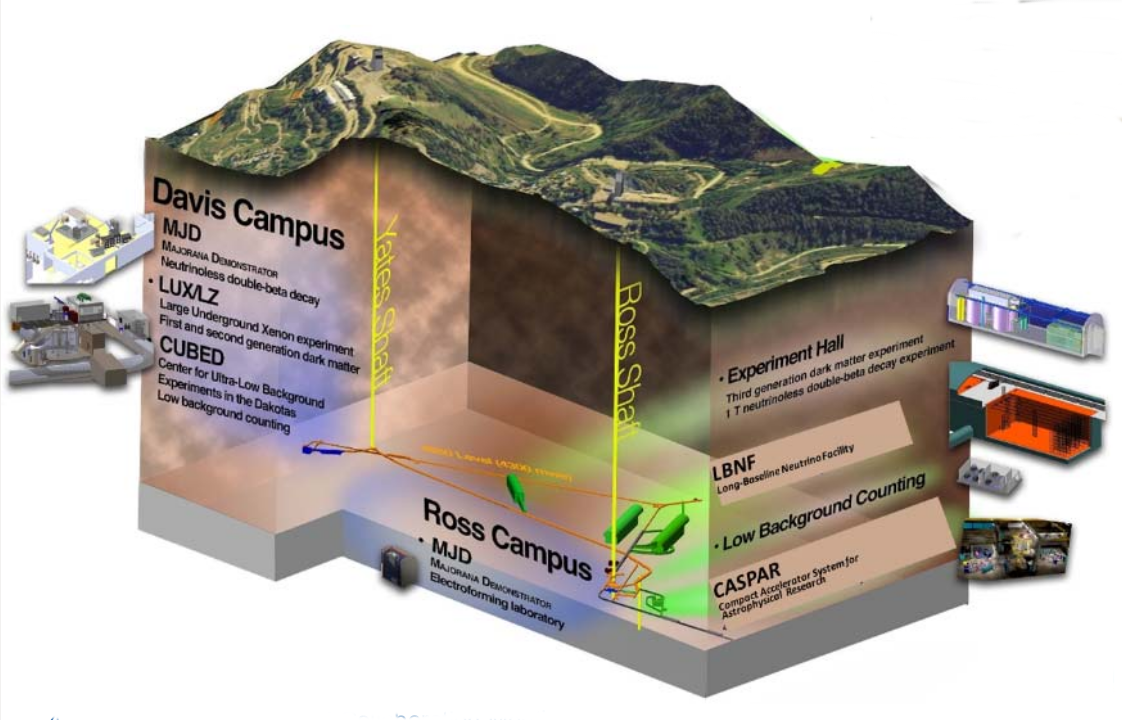
\includegraphics[width=0.98\textwidth, keepaspectratio=true]{figs/farDetector_SanfordUndergroundResearchFacility.png}
\end{figure}

\begin{figure}
\caption{Sanford Underground Research Facility (SURF)}
\label{fig:farDetector_SURF2}
\centering
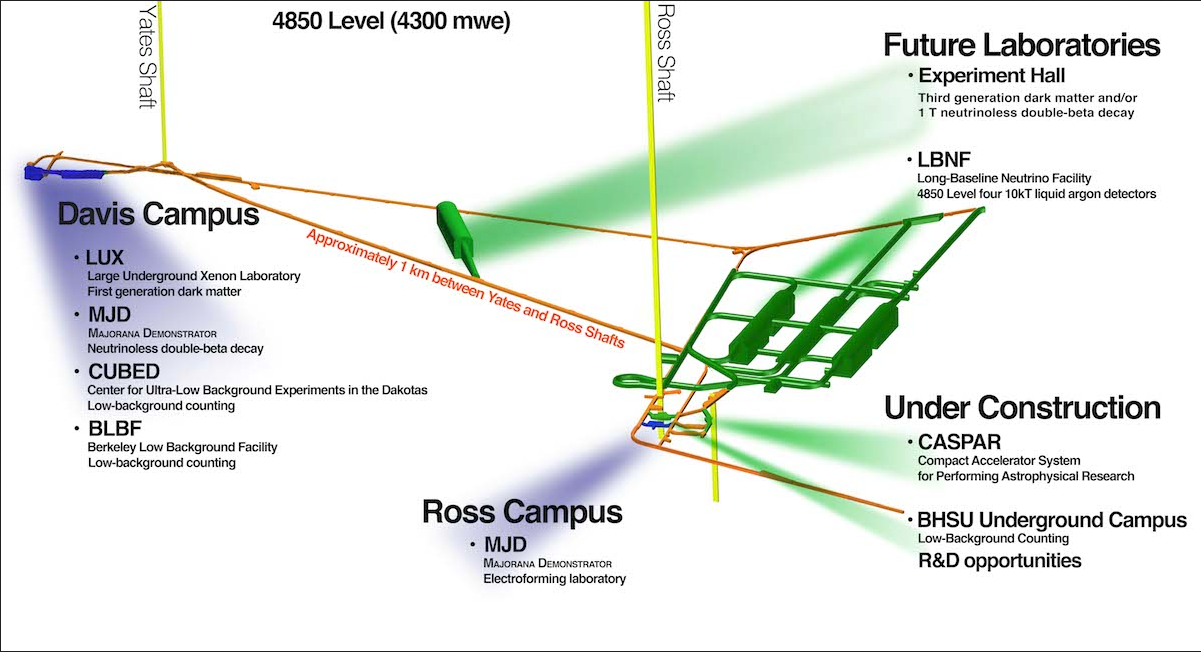
\includegraphics[width=0.98\textwidth, keepaspectratio=true]{figs/farDetector_wholeLab.png}
\end{figure}

\begin{SCfigure}
% side caption
\caption{The scheme of the cross section of the LArTPC for far detector of the DUNE. Source of figure: \cite{ref_LBNFdoc_volume-detectors}}
\label{fig:farDetector_TPC}
\centering
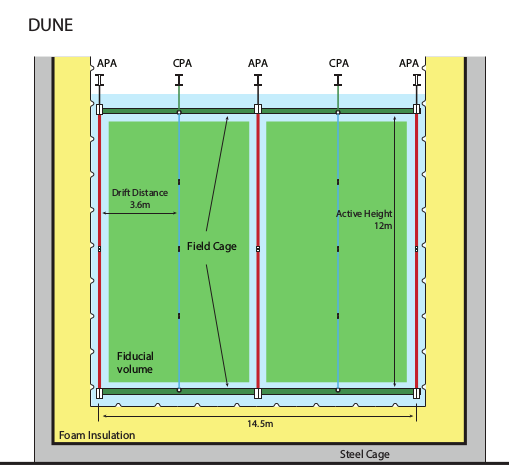
\includegraphics[width=0.75\textwidth, keepaspectratio=true]{figs/farDetector_TPC.png}
\end{SCfigure}

The liquid argon TPC is the main working volume of the detector. The chamber is merged into the liquid argon at tempetature of 89 K. On the figure \ref{fig:farDetector_TPC} the cathod plane assemblies (CPAs) and the anode plane assemblies (APAs) are shown. The voltages on the APAs and the CPAs are applied in such a way to create uniform electric field between anode and cathod planes. Charged particle travelling through the electron field ionizes argon atoms. Electrons induced in the ionization process drift to the APAs and produce signal on the readout electronic elements.
The important requirements to the TPC include:

\begin{itemize}
  \item be able to perform electron/photon discrimination
  \item wire sag shouldn't affect the position and energy resolutions
  \item discriminate electrons coming from photon conversion from primary electrons
  \item has good performance in measurements of high-energy and low-energy tracks
  \item make sure that materials used wouldn't contaminate high purity argon
\end{itemize}

% [Not sure whether it's good idea to place data aquisition system here, paper should concentrate on physics and major detector schemes]
%The scheme of the data aquisition system is showm on figure \ref{fig:LBNF_DAQ}. The data aquisition is performed in two steps. First, data are triggered by software trigger farm. Then the data which passed trigger requirement are collected.

%\begin{figure}
%\caption{Block Diagram of the Data Aquisition System for the Far Detector of DUNE}
%\label{fig:LBNF_DAQ}
%\centering
%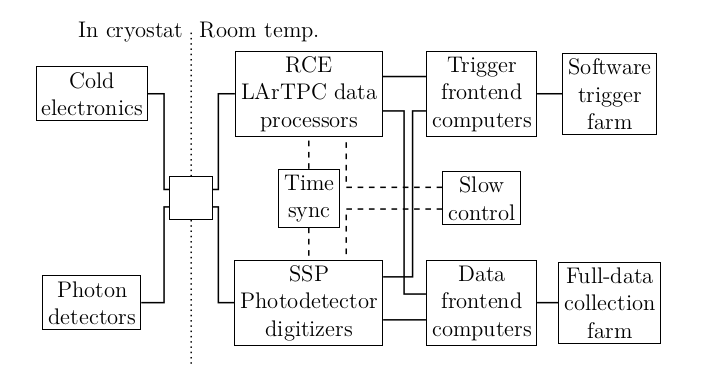
\includegraphics[width=0.70\textwidth, keepaspectratio=true]{figs/LBNF_DAQ.png}
%\\The scheme of the cross section of the LArTPC for far detector of the DUNE compared to LBNE (old experiment).   
%\end{figure}

\subsection{LBNF compared to the other long baseline neutrino oscillation experiments}
The review article \cite{ref_LBN_OscExpReview} describes beams and detectors of the long baseline neutrino experiments KEK \cite{ref_KEK}, NuMI \cite{ref_NuMI}, CNGS \cite{ref_CNGS} and J-PARC \cite{ref_JPARC}. The main parameters, compared to those of the LBNF, are summarized in the table \ref{tab:compareExps}. Common in facility setups for all these experiments is that they all include neutrino beam production system incremented to large accelerator facility, tracking near detector allowing precise measurements of the initial beam parameters and large volume far detector. Japanese old experiment K2K which operated in 1999-2004 and it's update T2K use different starting poins (KEK and J-PARC) but the same far detector - Super-Kamiokande, which is 50 kilotonnes water Cherenkov detector. T2K, which already delivered many important results, including the first mearument of $\theta_{13}$, is currently operating and looking forward to perform part of the LBNF physics program too. T2K's baseline is 295 km. The experiment hosted in USA, the NuMI, as well as proposed LBNF, uses neutrino beams produced in Fermilab but it's far detector, MINOS, is located in Minnessota and the experiment's baseline is 735 km. The working volume of the MINOS is magnetized tracker and polysterene scintillator, totalling to 5.4 kilotonnes. The European experiment, the CERN Neutrinos to Gran-Sasso (CNGS), as one can tell from it's name, has it's neutrino beam produced in CERN and the neutrinos measured in Gran-Sasso, Italy. This experiment has two far detectors: fine-grained tracker OPERA and, as well as the DUNE far detector, the liquid argon time-projection chamber ICARUS. But the DUNE has much larger working volume: 4 caverns, 10 kilotonnes each, compared to 760 tonnes ICARUS. As for the beam power, the LBNF is planned to have 2MW while other operating experiments has only beam powers of few hundred Watts. Therefore, among the experiments discussed, the LBNF is going to have the longest baseline (1300 km), the highest beam power and the most sensitive detector (while Super-Kamiokande has larger volume, it's filled with water which is not as favorable for the neutrino detection as liquid argon, as discussed in the subsection "Far Detector"). These characteristics will allow the LBNF to perform more precise measurements than previous and currently existing experiments can do and become sensitive to effects which weren't observed before.

\begin{table}[h]
  \centering
  \begin{center}
  \caption{ Comparison of different long baseline neutrino oscillations experiments. Abbreviations and notations used in the table: CNGS - CERN Neutrinos to Gran-Sasso, PS - Proton Synchrotron, J-PARC - Japan Accelerator Resarch Complex, FNAL - Fermilab National Accelerator Laboratory, $E_p$ - proton energy, DUNE - Deep Underground Neutrino Experiment, FGD - Fine-Grained Detector, ChD - Cherenkov Detector, SuperK - Super-Kamiokande, MINOS - Main Injector Neutrino Oscillation Search, OPERA - Oscillation Project with Emulsion-tRacking Apparatus, ICARUS - Imaging Cosmic And Rare Underground Signals, LAr - liquid argon }
  \begin{tabular}{|c|c|c|c|c|c|}
              & KEK (K2K) & NuMI & CNGS & T2K & LBNF (DUNE)\\ \hline
     location & Japan  & Illinois - & Switzerland - & Japan & Illinois - \\ 
              &        & Minnesota & Italy &  & South Dakota\\ \hline
     accelerator & KEK PS  & FNAL & CERN's SPS & J-PARC & FNAL\\ \hline
     time of oper. & 1999-2004  & 2005-2012 & 2006-2012 & 2010- & future \\ \hline 
     beam power  &  5 kW  & 300-350 kW  & 300 kW & 750 kW & 2000 kW\\ \hline 
     $E_p$  & 12 GeV & 120 GeV & 400 GeV & 30 GeV & 60-120 GeV\\ \hline 
     baseline  & 250 km & 735 km & 730 km & 295 km & 1300 km\\ \hline 
%                & KEK (K2K)   & NuMI                & CNGS                & T2K         & LBNF (DUNE)\\ \hline
     near        & (water ChD) & MINOS               & (muon               & ND280       & DUNE (FGD)\\  
     detector(s) & (FGD)       & (track. and scint.) & detector)           & INGRID      & \\ \hline 
     ND mass     & 1 kt (ChD)  & 0.98 kt             &                     &             & \\ \hline 
     far         & SuperK      & MINOS               & ICARUS (LAr)        & SuperK      & DUNE (LAr)\\  
     detector(s) & (water ChD) & track. and scint.   & OPERA (FGD)        & (water ChD) & \\ \hline 
     FD mass     & 50 kt       & 5.4 kt              & 0.76 kt (ICARUS)   & 50 kt       & 40 kt\\ 
                 &             &                     & 1.25 kt (OPERA)    &             & \\ \hline 
 \end{tabular}
  \label{tab:compareExps}
  \end{center}
\end{table}



